\section{Angriffe gegen Verteiltes Lernen}\label{sec:angriffe_verteiltes_lernen}

Die Größe und Komplexität eines Machine Learning Modells korreliert mit dem Funktionsumfang der zu bewältigen Aufgabe.
Dies führt dazu, dass eine große Datenmenge und mehr Rechenleistung benötigt werden.
Ist eines dieser beiden Ressourcen knapp, können diese von mehreren Partnern geteilt werden.
Das Verteilte Lernen birgt jedoch einige besondere Risiken, welche im Folgenden detaillierter betrachtet werden.


Verteiltes Lernen, auch Federated Learning oder Collaborative Learning genannt, kann unterschiedlich durchgeführt werden. 
Diverse Parameter, beispielsweise wie oft Systeme ihre Änderungen übermittelt, können konfiguriert werden.
Jedoch ist eine wichtige Unterscheidung die Topologie des Systems, welche in Abbildung \ref{fig:federated_learning_topo} gezeigt werden.
Links sieht man ein System, welches einen zentralisierten Server benutzt. 
Die Clients, dargestellt durch Smartphones, berechnen mit ihren privaten Daten Gradienten, welche dann an einen zentralen Server übermittelt werden. 
Dort findet die Anpassung des Modells statt.
Rechts sieht man einen dezentralen Ansatz, bei dem Clients miteinander vernetzt sind und ihre Updates (z. B. Gradienten) untereinander austauschen \cite{P-89}. 

\begin{figure}[!htb]
    \centering
    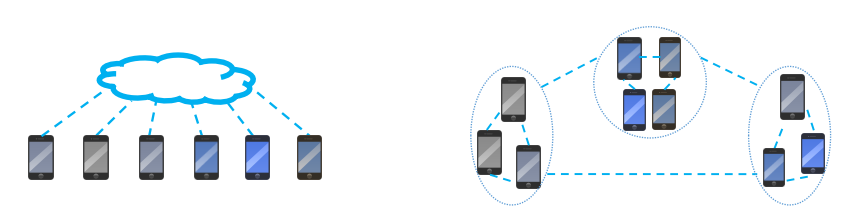
\includegraphics[width=12cm]{figures/federated_learning}
    \caption{Verteiltes Lernen Topologien \cite{P-89}}
    \label{fig:federated_learning_topo}
\end{figure} 

Melis et al. \cite{P-82} zeigen, dass Verteiltes Lernen anfällig für Membership Inference Attacken (siehe Kapitel \ref{sec:membership_inference}) und Property Inference Attacken (siehe Kapitel \ref{sec:property_inference}) sind.
Ein Membership Inference Angriff kann durchgeführt werden, indem die Gradienten der Eingabeschicht eines Neuronalen Netzes beobachtet werden. 
Bei Textmodellen beispielsweise, ist es oftmals der Fall, dass die Worte bzw. Tokens in einen Vektor übertragen werden. 
Dieser Vektor enthält dabei die Information, welche Knoten der ersten Schicht aktiviert sind. 
An besagten Stellen der ersten Schicht, sind die Gradienten deshalb ungleich 0.
Durch diese Beobachtung kann ein Angreifer also feststellen, welche Wörter in einem Datenpunkt oder einem Batch aus Datenpunkten enthalten sind.
Für einen Property Inference Angriff, kann der Angreifer verschiedene Snapshots des gemeinsam trainierten Modells nutzen. 
Jeder dieser Snapshots wird zweimal separat weitertrainiert, einmal mit einem Datensatz, welcher die zu untersuchende Eigenschaft enthält und einmal mit einem Datensatz der diese nicht enthält.
Die Unterschiede von den ursprünglichen Snapshot-Modellen und den weitertrainierten Modellen sind folglich die Inputs und die Labels sind die Information, ob Daten mit der Eigenschaft oder ohne die Eigenschaft zum Lernen genutzt wurden.
Damit kann nun ein Meta-Klassifikator trainiert werden, der vorhersagt, ob ein Modell weitertrainiert wurde, mit Daten, welche die zu untersuchende Eigenschaft enthält.
Bei jedem Update des gemeinsam gelernten Modells kann dieser Meta-Klassifikator genutzt werden.


Zhu et al. \cite{P-18} beschrieben einen Angriff auf Verteilte Systeme, welcher Deep Leakage genannt wird.
Der Angriff funktioniert sowohl bei einer zentralisierten als auch einer dezentralisierten Topologie. 
Beim zentralisierten System muss der Angreifer jedoch Zugriff auf den zentralen Server haben, beim dezentralisierten System reicht es, ein Teilnehmer zu sein.
Dies liegt daran, dass die Gradienten (bzw. eine Gradientenmatrix) mit dem Angreifer geteilt werden müssen, damit der Angriff funktioniert.
Im Laufe des Trainingsprozesses werden mehrfach Gradienten dem Angreifer übergeben, und für jeden Austausch, können die eingegebenen Trainingsdaten ermittelt werden.
Um den Angriff für eine Gradientenmatrix durchzuführen, wird initial ein Eingabevektor generiert.
Dieser wird durch das gemeinsam zu trainierende Modell interferiert, der Wert der Verlustfunktion bestimmt und anschließend durch das Modell backpropagiert.
Anstatt jedoch die Gewichte der Knoten des Modells anzupassen, werden nur die Werte des Eingabevektors iterativ (multipliziert mit einer festgelegten Lernrate) angepasst, sodass sich die Gradienten des Eingabevektors der geteilten Gradientenmatrix annähern.
Durch diese Angleichung, wird der ursprünglich initial gesetzte Eingabevektor immer ähnlicher zu den originalen Trainingsdaten, die ein anderer Nutzer des verteilten Systems zum Training genutzt hat.
Mit dieser Attacke, konnten die Autoren zeigen, dass die rekonstruierten Bilder nahezu (bis auf einige Pixel) identisch zu den Originalbildern sind. 
Abbildung \ref{fig:deep_leakage} zeigt einer Gegenüberstellung der Bilder.
Die Bilder können ebenfalls rekonstruiert werden, wenn mehrere Bilder in Batches zum Training genutzt werden.

\begin{figure}[!htb]
    \centering
    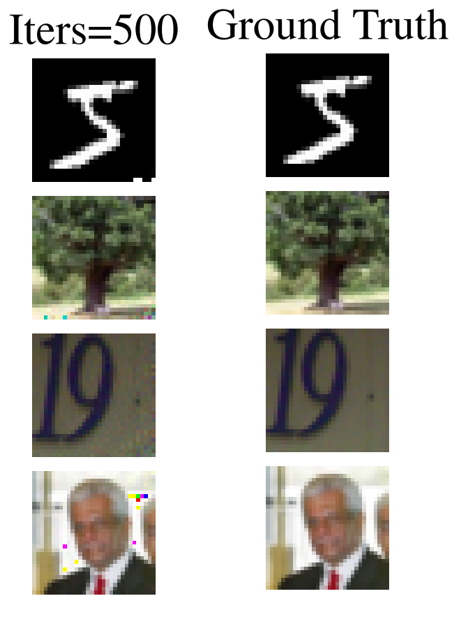
\includegraphics[width=6cm]{figures/deep_leakage}
    \caption{Rekonstruktion durch Deep Leakage \cite{P-18}}
    \label{fig:deep_leakage}
\end{figure} 

Zhao et al. \cite{P-19} optimierten den Deep Leakage Angriff, indem ein zusätzlicher Schritt in den Algorithmus eingefügt wird.
Dieser beinhaltet, dass zuerst das Label des Datenpunktes herausgefunden wird, von dem die Gradienten stammen.
Dies kann dadurch ermittelt werden, dass die Kostenfunktion eines Outputs bei der richtigen Klasse den Wertebereich (-1,0) annimmt und bei den falschen Klassen den Wertebereich (0,1), sofern keine Quadrierung stattfindet.
Der initiale Eingabevektor hat nun von Beginn an das richtige Label. 
Dadurch werden weniger Iterationen benötigt, um Daten zu rekonstruieren.


Hitaj et al. \cite{P-81} zeigen einen alternativen Angriff.
Bei diesem Szenario einigen sich die Trainingsteilnehmer darauf, von welchen Klassen sie jeweils Daten haben und entsprechend auch welche Sie davon im gemeinsamen Modell trainieren.
Klassen können sich unter den Teilnehmern überlappen, sodass mehrere Teilnehmer diese Klasse trainieren können.
Jedoch braucht der Angreifer eine Klasse, die außer ihm niemand hat.
Diese muss nicht wirklich in den Daten vorkommen, sondern es geht darum, dass kein anderer Teilnehmer die Klassifikation dieser Klasse beeinflusst.
Zur Durchführung des Angriffs, wird das Modell wie geplant trainiert, bis eine gewisse Güte erreicht ist.
Der Angreifer versucht nun, Daten einer Klasse zu rekonstruieren, die nur von anderen Teilnehmern bespielt wurde.
Dazu wird ein Generative Adversarial Network \cite{P-86} genutzt.
Dabei handelt es sich um eine Architektur, welche sich aus zwei Modellen, einem Generator und einem Discriminator, zusammensetzt.
Der Discriminator entscheidet dabei, ob die Daten, die vom Generator erzeugt werden, echt oder unecht sind. 
In diesem Angriff wird als Discriminator das gemeinsam gelernte Modell genutzt, welches vorhersagt, ob die Daten Teil der angegriffenen Klasse sind oder nicht.
Der Generator wird vom Angreifer trainiert, indem er das gemeinsame Modell auch durch den Generator backpropagiert.
Diese erzeugten Daten, kann der Angreifer der Klasse zuordnen, die außer ihm niemand trainiert. 
Daduruch werden andere Teilnehmer gedrängt, mehr oder öfters Daten für die angegriffene Klasse preis zu geben, da das gemeinsame Modell nicht mehr zwischen der angegriffenen Klasse und der zugeordneten Klasse des Angreifers unterscheiden kann.
Anschließend kann der Angreifer erneut den Generator verbessern.
Anzumerken ist hierbei noch, dass der Generator nicht die Trainingsdaten im Detail rekonstruiert, sondern nur Daten erzeugt, welche der gleichen Klasse zugeordnet werden können.
Die Autoren zeigen jedoch, dass bei Bildern eine erkennbare Ähnlichkeit vorhanden ist.